%---------------------------------------------------------------------------%
%->> Backmatter
%---------------------------------------------------------------------------%
%->> Question
%---------------------------------------------------------------------------%
\lecture{Research Presentation}{lec_present_question}
%---------------------------------------------------------------------------%
{%
\begin{frame}[plain]
    \begin{center}
        {\large\bfseries {Thank you for your attention!}}
    \end{center}
    \tikzart[t=p,x=0,y=-4,w=4]{bonn-logo}
    \addtocounter{framenumber}{-1}% modify the counter to exclude a frame from total count
\end{frame}
}
%---------------------------------------------------------------------------%
%->> Appendix
%---------------------------------------------------------------------------%
\lecture{Research Presentation}{lec_present_appendix}
%---------------------------------------------------------------------------%
%\appendix% begin appendix
%\newcounter{finalframe}% define a new counter
%\setcounter{finalframe}{\value{framenumber}}% save regular slides counter
%---------------------------------------------------------------------------%
%\section{\appendixname}% the end page.
%\frame{\tableofcontents}% outline for appendix
%---------------------------------------------------------------------------%
%\subsection{Classic Beamer Style}
%---------------------------------------------------------------------------%
\begin{frame}[fragile]
\frametitle{Appendix}
    \begin{figure}[b]
        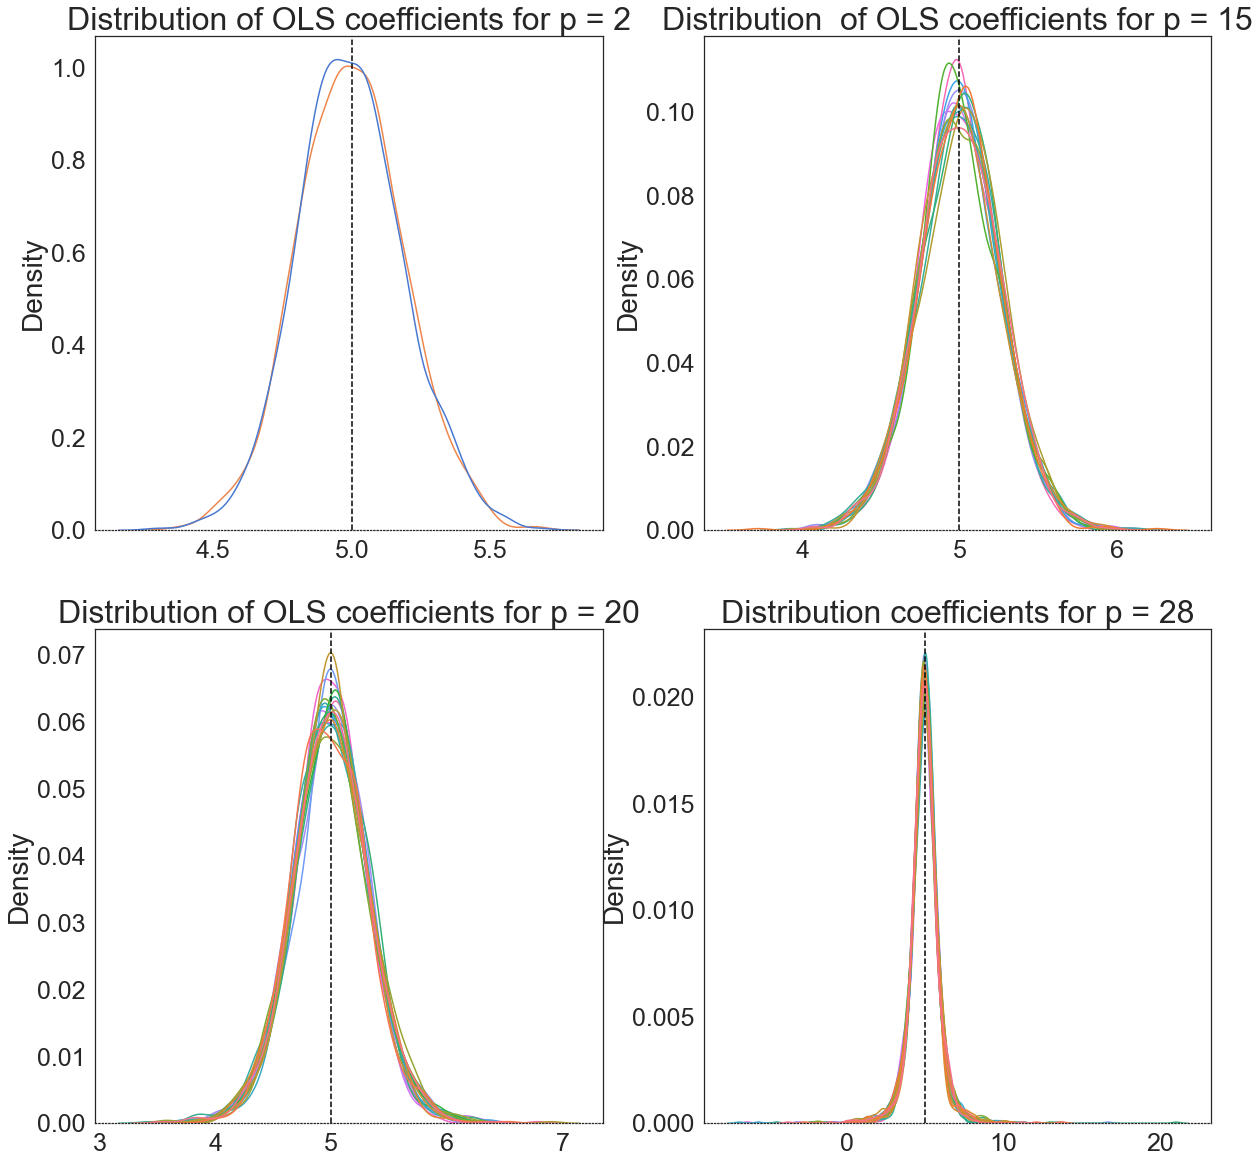
\includegraphics[scale=0.17]{Img/ols_distr.png}
        \centering
    \end{figure}
\end{frame}
%---------------------------------------------------------------------------%
\begin{frame}[fragile]
    \frametitle{Appendix}
    \begin{figure}[c]
        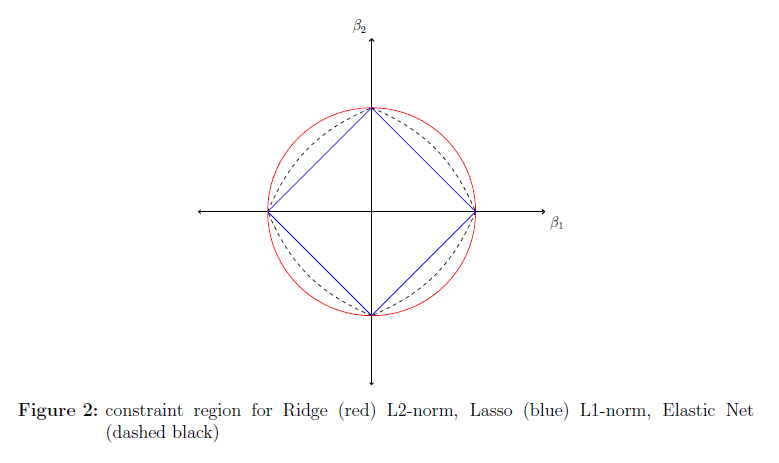
\includegraphics[scale=0.57]{Img/constraints.png}\hspace{-1.2cm}
        \centering
    \end{figure}
\end{frame}
%---------------------------------------------------------------------------%
\begin{frame}[fragile]
    \frametitle{Appendix}
    \begin{figure}[b]
        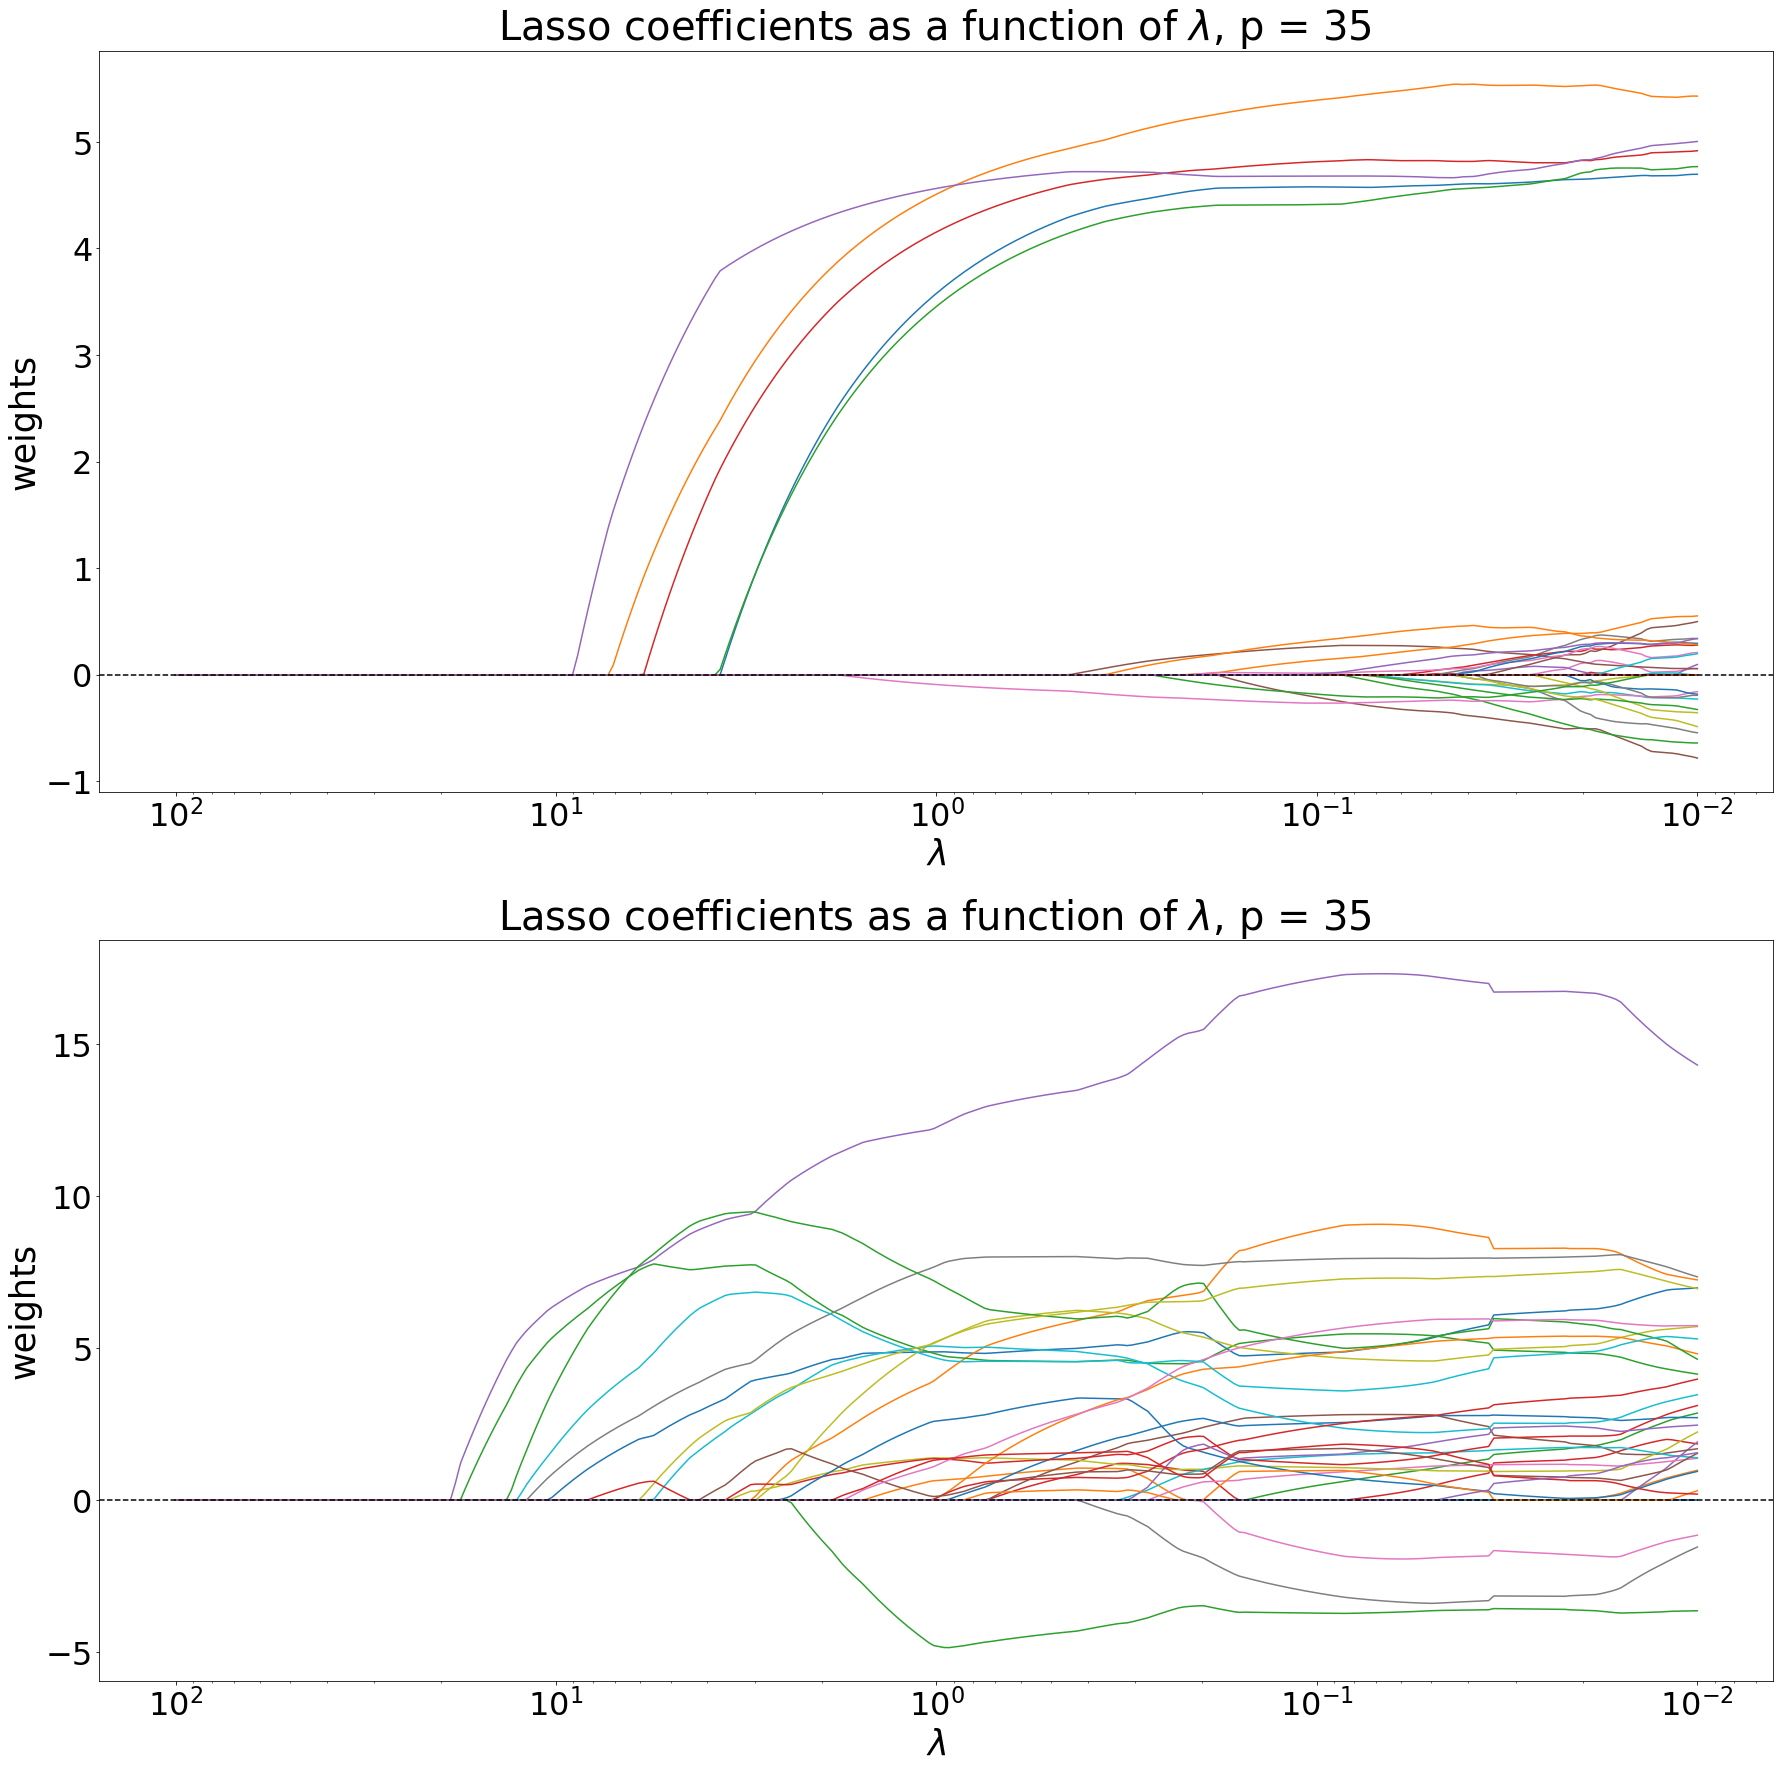
\includegraphics[scale=0.13]{Img/lasso_plot_betas.png}
        \centering
    \end{figure}
\end{frame}
%---------------------------------------------------------------------------%
\begin{frame}[fragile]
    \frametitle{Appendix}
    \begin{itemize}
        \item We used a \textit{10-fold cross validation} approach to find the optimal value of the tuning parameter.
    \end{itemize}
    \begin{align}
    \label{}
    CV_{(k)}=\frac{1}{k}\sum_{i=1}^{k} \: MSE_i
    \end{align}
    \begin{itemize}
        \item We identify the model with the lowest test error.
        \item We identify the $\lambda$ value that minimizes the MSE and then plug it back into the model of interest.
    \end{itemize}
\end{frame}
%---------------------------------------------------------------------------%
\begin{frame}[fragile]
    \frametitle{Appendix}
    \textbf{Least-angle regression (LARS) (\cite{efron2003lars})} \\
    \begin{itemize}
        \item Provides an extremely efficient algorithm for computing the entire lasso path.
        \item Lasso is a variant of the LARS procedure.
        \item LARS algorithm:
        \begin{enumerate}
            \item Standardize predictors.
            \item Find predictor $x_j$ that is most correlated with $y$.
            \item Move $\beta_j$ from 0 towards least-squares coefficient until  $x_k$ has as much correlation with the current residual as does $x_j$.
            \item Move $\beta_j$ and $\beta_k$ in the direction of the joint least squares coefficient of the current residual on ($x_j$, $x_k$), until $x_l$ has as much correlation with the current residual.
            \item Continue until all $p$ have been entered.
            \item \textit{If a non-zero coefficient hits zero, drop the corresponding variable from the active set of variables and recompute the current joint least squares direction.}
        \end{enumerate}
    \end{itemize}
\end{frame}
%---------------------------------------------------------------------------%
\lecture{Research Presentation}{lec_present_ref}
%---------------------------------------------------------------------------%
\subsection{References}
%---------------------------------------------------------------------------%
\begin{frame}[allowframebreaks]
    \frametitle{References}
    \nocite{*}
    \printbibliography[heading=none]%
\end{frame}
%---------------------------------------------------------------------------%
%\setcounter{framenumber}{\value{finalframe}}% rectify the slides counter
%---------------------------------------------------------------------------%
